\chapter{Responsive Information Visualization}

A responsive visualization is a visualization that adapts to the properties of the device used to access it. Similar to responsive design, the need for responsive visualizations arises from the growing variety of devices used to consume content and the physical differences between them. On the web, visualizations are significant blocks of content that are embedded into documents. These blocks of content must not be ignored when a web page adhering to the principles of responsive web design is to be created. Visual elements require proper sizing and spacing to be of value. Merely scaling visualizations to fit into their allocated space is not sufficient to provide a seamless experience to users, as has already been discussed in Section \ref{sec:RWD}. Another factor that is often ignored is the different methods of interaction inherent to specific types of devices. In addition to enabling these device-specific types of interaction, web designers need to adjust visualizations accordingly to support them as well as possible. An example for such a necessary adjustment would be to ensure that data points remain selectable on less precise input devices, such as touchscreens, by reducing the data density and increasing the size of individual elements. The goal of responsive visualizations is to alter them depending on the characteristics of the consuming device to ensure an optimal trade-off between the density of graphical elements and the messages they aim to deliver \parencite{DesignPatternsTradeOffsRespVis}. 

The topic of responsive visualization only came up in recent years, with \cite{RespVis} being one of the first academic works exploring it. Earlier works \parencite{BuildingRespDataVisForTheWeb,LearningRespDataVis} exist, but they strongly focus on the aspect of software development and do not go much into detail on how to properly design responsive visualizations.  For design-related fields, it is generally helpful to study existing solutions and better define the design space by creating taxonomies of currently used techniques and recurring patterns. In the case of responsive visualization, some such works already exist \parencite{TechniquesForFlexibleRespVisDesign,DesignPatternsTradeOffsRespVis,RespVisSurvey} and the various patterns defined in them, including some representative examples, are discussed in the following sections.

\section{Responsive Visualization Patterns}

Patterns are templates for solving recurring problems. The core problem to solve when designing responsive visualizations is to optimize the trade-off between the visual density of components and the messages that the visualization aims to convey \parencite{DesignPatternsTradeOffsRespVis}. Many techniques can be applied to solve that problem by using the available screen space as efficiently as possible. Various authors have analyzed many existing visualizations to identify recurring patterns, and they formulated different taxonomies based on their results.

\cite{RespVisSurvey} have conducted a survey under close supervision by Keith Andrews \parencite{RespVis} identifying nine common patterns that reoccurred in several solutions. Slightly reworded, these patterns are: (1) rotate axis labels, (2) remove axis ticks, (3) modify strings, (4) transpose chart, (5) reposition components, (6) zoom, (7) filter, (8) modify data density and (9) modify chart type. Compared to other works, they did not categorize the techniques they found according to multiple dimensions. Rather than that, they created a collection of specific patterns and, even though they are a good collection on which to base further research, they are not comprehensive enough to cover all the techniques that can be applied to increase the responsiveness of a chart. An example of a technique that can not be derived from these patterns is the adding and removing of components, such as in the example of a responsive line chart by \cite{RespVis}, in which the chart's axes were removed on narrow screens. These patterns also do not consider any adaptations of interactions, which should not be ignored when talking about responsive design.

A more comprehensive categorization of responsive techniques was created by \cite{TechniquesForFlexibleRespVisDesign}. They state that responsive techniques can be described by a set of five actions that are applied to different components. These actions are: (1) resize, (2) reposition, (3) add, (4) modify and (5) remove. A sixth action that refers to not changing a component has also been defined in their work, but this is deemed a non-technique and therefore left out. They list a collection of eleven components on which these actions can be performed, though they do not claim this list to be exhaustive. For the sake of completeness, the components they identified are: (1) axis, (2) axis labels, (3) axis ticks, (4) gridlines, (5) legend, (6) data, (7) marks, (8) labels, (9) title, (10) view, and (11) interaction. It should be noted that some combinations of actions and components do not make sense and therefore do not occur in practice. It is, for example, not possible to resize interactions or reposition data. \cite{TechniquesForFlexibleRespVisDesign} performed their research following a desktop-first approach of responsive design because the interviews they conducted with visualization authors revealed a strong inclination towards this approach. They found that when adapting desktop visualizations for narrow screens, it was much more common to remove elements (37.7\%) than to add them (11.3\%). Another one of their findings was that most visualizations (88.7\%) implemented no change at all for their interactions, while some (10\%) even removed interactive capabilities completely. On the other hand, a few visualizations (5.6\%) improved the experience of mobile users by adapting interactions accordingly.

The most detailed research on patterns in responsive visualization design was performed by \cite{DesignPatternsTradeOffsRespVis}. Similar to \cite{TechniquesForFlexibleRespVisDesign}, they formulate the strategies they found in terms of the same two dimensions: targets, representing what entity is changed, and actions, representing how entities are changed. Apart from the grouping of specific targets into five distinct categories shown in Table \ref{tab:PatternsTargets}, the major difference to the taxonomy defined by \cite{TechniquesForFlexibleRespVisDesign} is the increased level of detail that is put into the definition of actions. Instead of describing actions as general editing operations (resize, reposition, add, etc.), they are defined by how exactly they affect their targets. The action dimension consists of five categories that are split into further subcategories, shown in Table \ref{tab:PatternsActions}. These subcategories are defined as operations with distinct input and output states. This ensures that actions can be inverted, and that these patterns can be applied in both a desktop-first and a mobile-first design approach. Categorizing techniques using these dimensions, the authors identified a total of 76 viable strategies, with some of them not being used in the visualizations they studied and excluding others that are by definition not possible. Listing all these strategies here is outside the scope of this work, but the explorable online gallery by \cite{DesignPatternsTradeOffsRespVisGallery} contains examples demonstrating all these patterns and shall be referred to for further research.

\begin{table}[tp]
    \centering
    \begin{tabularx}{\linewidth}{| l | X |}
        \hline
        \textbf{Category} & \textbf{Description} \\ \hline
        Data & Data is the information that is encoded in a visualization. This category includes targets such as data records, data fields, or levels of hierarchy in the data.  \\ 
        \hline
        Encoding & Encodings are the visual forms in which data is represented.  \\ 
        \hline
        Interaction & Interactions are the way that users can engage with visualizations. This category includes targets such as interaction triggers, interaction feedback and interaction features. \\ 
        \hline
        Narrative & This category groups targets based on the story a visualization should convey. It contains targets such as the presented sequence of information (views and states) and the information itself in the form of annotations, emphases, and texts. \\ 
        \hline
        References/Layout & References represent additional information that makes visualizations easier to understand, and a layout describes how the individual visual components are placed. \\ 
        \hline
    \end{tabularx}
    \caption[Targets of Responsive Visualization Patterns]
    {
        This table shows the different target categories of responsive visualization patterns. A target of a responsive visualization pattern defines the entity that is changed by it.
        \imgcredit{Table adapted from \cite{DesignPatternsTradeOffsRespVis}}
    }
    \label{tab:PatternsTargets}
\end{table}

\begin{table}[tp]
    \centering
    \begin{tabularx}{\linewidth}{| l | X |}
        \hline
        \textbf{Category} & \textbf{Description} \\ \hline
        Recompose & Actions that affect the existence of targets. Includes remove, add, replace and aggregate actions. \\
        \hline
        Rescale & Actions that affect the size of targets. Includes reduce width, simplify labels and elaborate labels actions. \\
        \hline
        Transpose & Actions that affect the orientation of targets. Includes serialize, parallelize and axis-transpose actions. \\
        \hline
        Reposition & Actions that affect the position of targets. Includes externalize, internalize, fix, fluid and relocate actions. \\
        \hline
        Compensate & Actions that compensate for loss of information. Includes toggle and number actions. \\
        \hline
    \end{tabularx}
    \caption[Actions of Responsive Visualization Patterns]
    {
        This table shows the different action categories of responsive visualization patterns. The action of a responsive visualization pattern defines how exactly it affects an entity.
        \imgcredit{Table adapted from \cite{DesignPatternsTradeOffsRespVis}}
    }
    \label{tab:PatternsActions}
\end{table}

\section{Responsive Visualization Examples}

The goal of this section is to provide the reader with some demonstrative examples of responsive visualizations. The figures in this section were taken from external scientific sources that put most of their effort into demonstrating responsive visualization patterns rather than communicating messages in the data they used. Because of this, some figures below are lacking essential features, such as titles and axes descriptions, that would usually be present in practice. The examples in this section are organized by chart type, with each paragraph describing some responsive patterns applicable to a certain type of chart. It would be an immense endeavor to bring examples for every pattern used for all types of charts, so only a subset that demonstrates some of the most frequently encountered patterns for frequently used types of charts will be summarized here.

The first types of charts that shall be discussed are a bar charts. They are among the most often encountered types of charts, accounting for 135 (= 36\%) of the 378 responsive charts studied by \cite{DesignPatternsTradeOffsRespVis}. Bar charts are usually used to visualize two-dimensional data, with one dimension being categorical and the other one being quantitative. Two additional variants of bar charts exist to visualize categorical datasets with multiple subdimensions: grouped bar charts \parencite{GroupedBar}, to compare subdimensions with each other, and stacked bar charts \parencite{StackedBar}, to compare part-to-whole relationships of the subdimensions. Even though responsive design of visualizations is slowly becoming more common, most charts found in today's web articles are still being created as static images \parencite{HBar,VBar,HVBar,MapBarLine}. A good example of a responsive bar chart has been created by \cite{RespVis} and can be seen in Figure \ref{fig:RespBarExample}. Bar charts are freely scalable by adjusting the width of individual bars \parencite{RespHBar,RespHBarHLine,RespHBars}, so they all can fit into their allocated space. When reducing the width of any type of chart past a certain point, the tick labels of the horizontal axis may start overlapping each other. This is why the reducing width pattern usually occurs together with the recompose axis ticks and simplify/elaborate axis labels patterns \parencite{RespHBars,RespHBarHLine,RespVBar}. Another effective pattern for solving overlapping of tick labels is to rotate them by up to 90 degrees to make them take up less horizontal space \parencite{RespVis}. If there is too much data to fit into the available width, the chart can be transposed and grown to as much height as necessary \parencite{RespVis}. Doing this is advisable over simply extending the width of the chart past the viewport because vertical scrolling is easier to achieve than horizontal scrolling. When reducing the size of charts that contain annotations, similar patterns than those targeting tick labels can be applied to avoid the annotations from overlapping. Annotations can simply be removed \parencite{RespHStackedBar,RespHLineHStackedBar}, or they can be simplified and relocated \parencite{RespVBar}.

\begin{figure}[tp]
\centering
\subfloat[][%
70rem
]
{%
\includegraphics[width=0.47\linewidth]
{images/resp-bar-1.png}%
\label{fig:RespBarExample1}%
}
\hfill
\subfloat[][%
50rem
]
{%
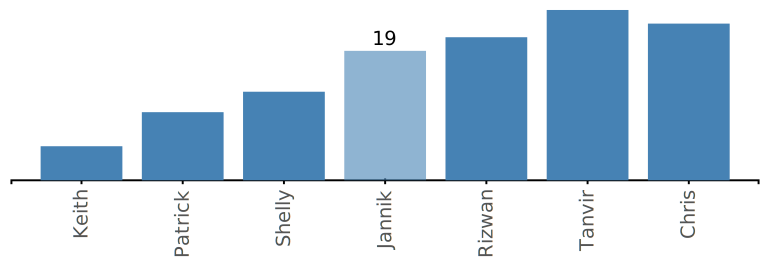
\includegraphics[width=0.33\linewidth]
{images/resp-bar-2.png}%
\label{fig:RespBarExample2}%
}
\hfill
\subfloat[][%
30rem
]
{%
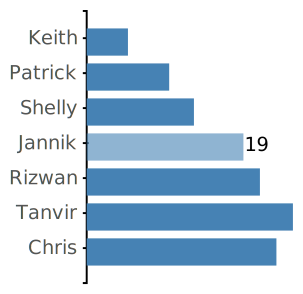
\includegraphics[width=0.2\linewidth]
{images/resp-bar-3.png}%
\label{fig:RespBarExample3}%
}
\caption[Responsive Bar Chart Example]
{
An example of a responsive bar chart at different display widths. \subref{fig:RespBarExample1} Axis tick labels are aligned horizontally. \subref{fig:RespBarExample2} Axis tick labels are aligned vertically. \subref{fig:RespBarExample3} Chart is transposed.
\imgcredit{Screenshots of \cite{RespVis} created by the author of this thesis. Used with kind permission by Keith Andrews.}
}
\label{fig:RespBarExample}
\end{figure}

The second most frequent types of responsive charts according to the responsive visualization gallery created by \cite{DesignPatternsTradeOffsRespVis} are line charts, which amount to 98 (= 26\%) out of the 378 responsive visualizations in the gallery. Line charts are used to show trends in two-dimensional datasets by plotting them as points that are then connected by lines. They can be extended to compare trends in multiple dimensions with each other by drawing additional points and lines for every additional dimension that shall be compared. Many line charts on the web are still published in non-responsive forms \parencite{HLine,HLine2}, though some web authors already took the extra effort to make their charts responsive. The minimum that can be done to make a line chart responsive is to reduce their width \parencite{RespRadialScatterHLine} by shrinking the horizontal distance between neighboring points. This usually occurs together with the recomposition and simplification of horizontal ticks. If the chart contains annotations, it may also be necessary to recompose, relocate, and simplify them as well \parencite{RespHLines,RespHLine,RespHBarHLine,RespHLineHStackedBar}. A good demonstration of which responsive patterns can be applied to make a line chart responsive is shown in the responsive line chart created by \cite{RespVis} that can be seen in Figure \ref{fig:RespLineExample}. In addition to the recomposition of ticks, tick labels are rotated to reduce their required horizontal space. For exceptionally limited space, it can make sense to remove the axes of a line chart entirely and turn it into a sparkline. However, it should be noted that by doing this, the consumer of the visualization looses a lot of information about the type and scale of the chart's dimensions. This technique should therefore only be applied in cases where no other pattern is applicable or if the trend in the data is the most important message to convey. It is rare to encounter transposed versions of line charts, though the transposing could benefit heavily annotated line charts \parencite{VLine}. Applying a transpose pattern would allow the chart to take up as much vertical space as necessary to neatly fit all the annotations without requiring the consumer to scroll horizontally.

\begin{figure}[tp]
\centering
\subfloat[][%
65rem
]
{%
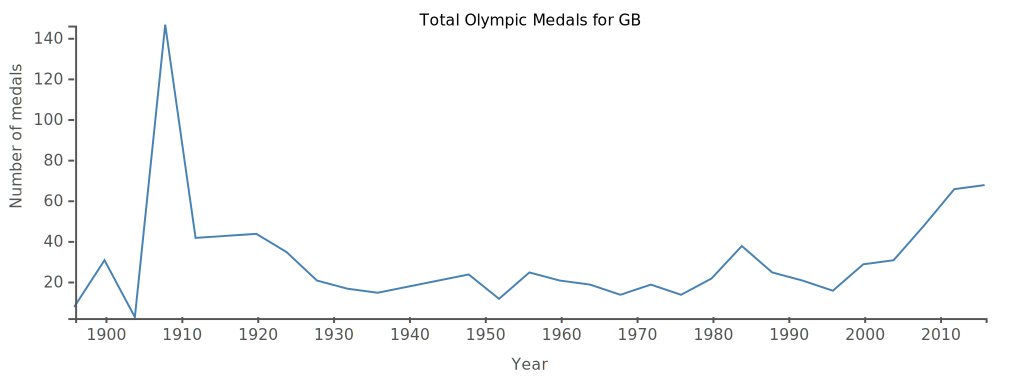
\includegraphics[width=0.52\linewidth]
{images/resp-line-1.png}%
\label{fig:RespLineExample1}%
}
\hfill
\subfloat[][%
40rem
]
{%
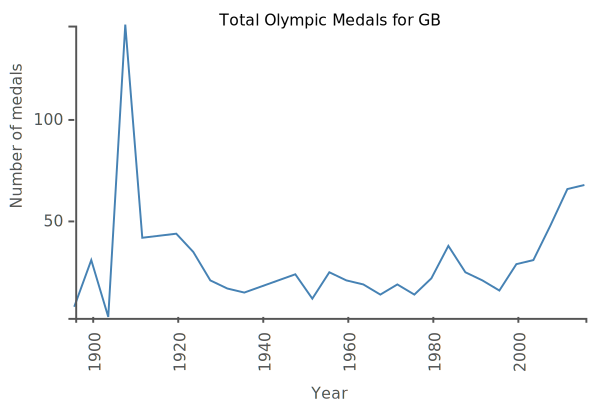
\includegraphics[width=0.31\linewidth]
{images/resp-line-2.png}%
\label{fig:RespLineExample2}%
}
\hfill
\subfloat[][%
20rem
]
{%
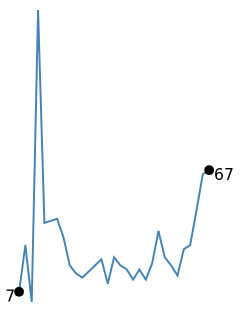
\includegraphics[width=0.16\linewidth]
{images/resp-line-3.png}%
\label{fig:RespLineExample3}%
}
\caption[Responsive Line Chart Example]
{
An example of a responsive line chart at different display widths. \subref{fig:RespLineExample1} Maximum width configuration is shown. \subref{fig:RespLineExample2} Axis ticks are thinned out and labels are rotated. \subref{fig:RespLineExample3} Axes are removed, turning the chart into a sparkline.
\imgcredit{Screenshots of \cite{RespVis} created by the author of this thesis. Used with kind permission by Keith Andrews.}
}
\label{fig:RespLineExample}
\end{figure}

Scatterplots are also among the rather frequently encountered types of responsive charts, amounting to 26 (= 7\%) of the 378 responsive charts contained in the gallery by \cite{DesignPatternsTradeOffsRespVis}. A scatterplot is a visualization that represents two-dimensional data as points in a Cartesian coordinate system. There are plenty of examples of scatterplots that are merely being published as static images \parencite{Scatter,Scatter2}, even though responsive versions can also already be observed occasionally. The first step to making scatterplots responsive is to reduce their width to fit them into the space available for them. As for other types of charts, care must be taken to avoid overlapping of labels and annotations by applying recomposition, relocation and simplification patterns \parencite{RespScatter,RespScatter2}. To counteract the increased cramming of points when reducing the size of their container, various interaction features are usually implemented in scatterplots that help consumers in making sense of the represented data. The most useful interaction features in these charts are elaborative zooming interactions and the explorative panning interactions. In addition to zooming and panning, \cite{RespVis} employs additional methods that reduce overlapping of individual points, such as fisheye distortion, Cartesian distortion or temporary displacements of points. An interesting technique for responsive visualizations that bases responsive configurations on a visualization's density rather than on its size has been introduced by \cite{NickRabinowitzRDV}. The benefit of this approach is that charts will also adapt to changing amounts of data and reconfigure their appearance accordingly. The patterns applied in the responsive scatterplot by \cite{NickRabinowitzRDV} that can be seen in Figure \ref{fig:RespScatterExample} are the recomposition of annotations to only show them for selected data records, and the switching of the encoding from a scatterplot to a heatmap for high densities. A good number of other techniques, such as for example the recomposition of data records, are also applicable to improve the responsiveness of scatterplots, but no examples for such patterns could be found. If the data that shall be encoded is inherently cyclic, a radial scatterplot, which is a polar coordinate system variant of a scatterplot, can be applied to better visualize this cyclic nature of the data \parencite{RespRadialScatterHLine}. 

\begin{figure}[tp]
\centering
\subfloat[][%
0.00005 points per pixel
]
{%
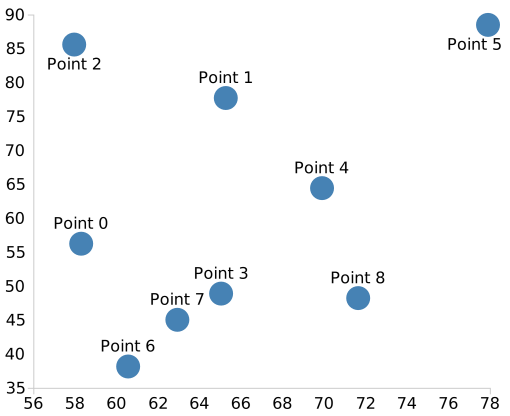
\includegraphics[width=0.33\linewidth]
{images/resp-scatter-1.png}%
\label{fig:RespScatterExample1}%
}
\hfill
\subfloat[][%
0.0007 points per pixel
]
{%
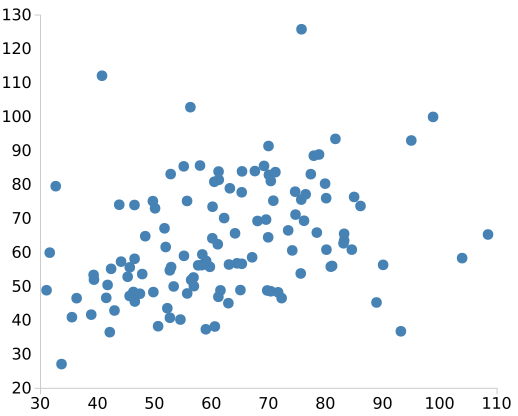
\includegraphics[width=0.33\linewidth]
{images/resp-scatter-2.png}%
\label{fig:RespScatterExample2}%
}
\hfill
\subfloat[][%
0.017 points per pixel
]
{%
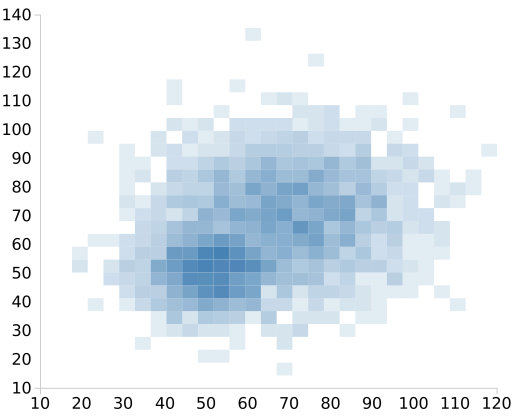
\includegraphics[width=0.33\linewidth]
{images/resp-scatter-3.png}%
\label{fig:RespScatterExample3}%
}
\caption[Responsive Scatterplot Example]
{
An example of a responsive scatterplot with increasing amount of data. The breakpoints on which the design changes are defined on the metric of data density (points per pixel) instead of on the width of the viewport as is usually the case. \subref{fig:RespScatterExample1} All points and their corresponding labels are shown. \subref{fig:RespScatterExample2} Point labels have been removed and are only shown for selected points. \subref{fig:RespScatterExample3} The scatterplot has been replaced by a heatmap to more efficiently display the large amount of data.
\imgcredit{Screenshots created by the author of this thesis. Visualization created by \cite{NickRabinowitzRDV}}
}
\label{fig:RespScatterExample}
\end{figure}

Even though parallel coordinates charts are rarely encountered in non-technical contexts, they are very popular when it comes to visualizing multidimensional data in visual analytics systems \parencite{HighD}. In these kinds of charts, multiple dimensions are rendered as parallel axes that are connected via paths. Each path represents an individual data record and its values in the corresponding dimensions. The axes of a parallel coordinates chart are typically laid out horizontally, meaning that the chart can be scaled down by reducing the distance between the individual axes. It might also be beneficial to apply previously mentioned axis-related patterns, such as rotating labels and recomposing ticks. Another technique that can be applied to make parallel coordinates charts more responsive is the successive hiding of dimensions based on their priorities. When automatically hiding dimensions, it is necessary to apply compensation patterns that give users additional controls that allow configuration of the displayed dimensions to override the system's hiding behavior. If reducing the chart's complexity is not a desirable approach, it can again be recommended to transpose the chart and expand it to whatever height necessary rather than cram too much information into the limited width available. An example of a responsive parallel coordinate chart incorporating some of these patterns can be seen in Figure \ref{fig:RespParCoordExample}.

\begin{figure}[tp]
\centering
\subfloat[][%
61rem
]
{%
\includegraphics[width=0.55\linewidth]
{images/resp-parcoord-1.png}%
\label{fig:RespParCoordExample1}%
}
\hfill
\subfloat[][%
50rem
]
{%
\includegraphics[width=0.45\linewidth]
{images/resp-parcoord-2.png}%
\label{fig:RespParCoordExample2}%
}
\hfill
\subfloat[][%
40rem
]
{%
\includegraphics[width=0.4\linewidth]
{images/resp-parcoord-3.png}%
\label{fig:RespParCoordExample3}%
}
\hfill
\subfloat[][%
30rem
]
{%
\includegraphics[width=0.3\linewidth]
{images/resp-parcoord-4.png}%
\label{fig:RespParCoordExample4}%
}
\hfill
\subfloat[][%
30rem with re-added dimensions
]
{%
\includegraphics[width=0.3\linewidth]
{images/resp-parcoord-5.png}%
\label{fig:RespParCoordExample5}%
}
\caption[Responsive Parallel Coordinates Chart Example]
{
An example of a responsive parallel coordinates chart at different display widths. \subref{fig:RespParCoordExample1} All dimensions are shown. \subref{fig:RespParCoordExample2} Dimensions are removed based on their priority and dimension labels are rotated by 45 degrees. Also, a dimensions toggle is shown that allows configuration of dimensions. \subref{fig:RespParCoordExample3} Further dimensions are removed. \subref{fig:RespParCoordExample4} Further dimensions are removed, and dimension labels are rotated by 90 degrees. \subref{fig:RespParCoordExample5} Dimension configuration panel is opened, and a dimension has been manually re-added.
\imgcredit{Screenshots of \cite{RespVis} created by the author of this thesis. Used with kind permission by Keith Andrews.}
}
\label{fig:RespParCoordExample}
\end{figure}

% \begin{figure}[tp]
% \centering
% \subfloat[][%
% 43rem
% ]
% {%
% \includegraphics[width=0.56\linewidth]
% {images/resp-radial-scatter-1.png}%
% \label{fig:RespRadialScatterExample1}%
% }
% \hfill
% \subfloat[][%
% 34rem
% ]
% {%
% \includegraphics[width=0.44\linewidth]
% {images/resp-radial-scatter-2.png}%
% \label{fig:RespRadialScatterExample2}%
% }
% \caption[Responsive Radial Scatterplot Example]
% {
% \TODO{Maybe remove this example because of copyright?}
% . \subref{fig:RespRadialScatterExample1} . \subref{fig:RespRadialScatterExample2} . \imgcredit{Screenshots made by the author of this thesis. Visualization created by \cite{LuringMinersToTheStars}}
% }
% \label{fig:RespRadialScatterExample}
% \end{figure}